\documentclass[a4paper,12pt]{article}
\usepackage[utf8x]{inputenc}
\usepackage[T1]{fontenc}

%\usepackage[T2A]{fontenc} % jei yra kirilica
\usepackage[hmargin={30mm,15mm},vmargin={20mm,20mm},bindingoffset=0mm]{geometry}
\usepackage[onehalfspacing]{setspace}
\usepackage[colorlinks=true, linkcolor=blue, citecolor=blue, urlcolor=blue, unicode]{hyperref}

%\parindent=7mm
\usepackage{graphicx}
\renewcommand{\refname}{Literatūros sąrašas} % article
%\renewcommand{\bibname}{Literatūros sąrašas} % report
\renewcommand{\contentsname}{Turinys}
\usepackage[T1]{fontenc} 

% Lukas paketai
\usepackage{eso-pic}
\usepackage{indentfirst}
\usepackage{setspace}
\usepackage{placeins}
\usepackage{booktabs}% http://ctan.org/pkg/booktabs
\usepackage{tabularx}% http://ctan.org/pkg/tabularx
\usepackage[parfill]{parskip}
\usepackage[unicode]{hyperref}
\usepackage{hyperref}
\usepackage{tocloft}
\usepackage{graphicx}
\newcommand\AtPageUpperRight[1]{\AtPageUpperLeft{%
   \makebox[\paperwidth][r]{#1}}}
\usepackage[dotinlabels]{titletoc}
\usepackage[capposition=top]{floatrow}
\hypersetup{
    colorlinks,
    citecolor=black,
    filecolor=black,
    linkcolor=black,
    urlcolor=black
}
\usepackage{secdot}




\begin{document}


\renewcommand{\cftdot}{.}	
\renewcommand{\cftsecleader}{\cftdotfill{\cftdotsep}}

\thispagestyle{empty} % nerasomas psl. nr


\begin{center}
 VILNIAUS UNIVERSITETAS 
 
MATEMATIKOS IR INFORMATIKOS FAKULTETAS

MATEMATINĖS INFORMATIKOS KATEDRA

\vspace{4cm}

Projekto vadovė \ \ \textbf{Aistė Čiplytė} \\
\textbf{Lukas Tutkus} \\
\textbf{Julius Daukšas} \\
\textbf{Dominykas Smaliukas} \\
\textbf{Robert Stankevič} \\

\vspace{0.2cm}

Bioinformatikos studijų programos grupė BioSawmill



\vspace{3cm}
\textbf{\Large Dvimatė pjovimo optimizacija}\\
\textbf{\Large Projekto planas}

\vfill

Vilnius \ \  2015
\end{center}



\clearpage

\tableofcontents
\clearpage
%\maketitle 
%\section*{Apžvalga}
%\addcontentsline{toc}{section}{Apžvalga} % rasoma turinyje
\section{Reikalavimai}

\begin{frame}
\centering

\label{my-label}
\begin{tabular}{|l|l|l|}
\hline
\textbf{ID}	& \textbf{Reikalavimai}							& \textbf{Moduliai}  \\ \hline

F1	& Registracijos forma									& 1	     		\\ \hline

F2	& Prisijungimo forma										& 1, 3			\\ \hline

F3	& Atsijungimo nuo sistemos mygtukas						& 1, 3			\\ \hline

F4	& Vartotojo slaptažodžio pakeitimo forma					& 1, 3			\\ \hline

F5	& Keisti paskyros duomenis	 	  						& 1, 3			\\ \hline 

F6	& Pjovimo optimizacijos duomenų įvedimo laukai			& 1, 3			\\ \hline

F7  & Papildomų standartinių panelių įvedimas 				& 1, 3			\\ \hline

F8	& Pjūvio plano informacijos apdorojimas					& 2				\\ \hline

F9	& Pjūvio plano optimizavimas           	   				& 2				\\ \hline

F10	& Optimizuotų pjūvio planų informacijos pateikimas		& 2     			\\ \hline

F11	& Optimizuotų pjūvio planų variantų pasirinkimas			& 1, 3			\\ \hline

F12	& Pasirinkto pjūvio planų ruošinių atsispausdinimas(??)	& 1, 3			\\ \hline

F13	& Pasirinkto pjūvio planų informacijos išsaugojimas(??)	& 1, 3			\\ \hline

F14	& Administratoriaus valdymo skydas	 	  				& 3				\\ \hline

F15	& Kalbos pasirinkimas(LT, EN)							& 1, 3			\\ \hline

NF1 & Užtikrinti kalbos pakeitimą							& 1, 3			\\ \hline

NF2 & Slaptažodžio ilgis nemažesnis nei 8 simboliai.			& 1, 3			\\ \hline 

NF3 & Prisijungimo duomenys vardas, paštas-unikalūs.			& 1, 3			\\ \hline 

NF3 & 
\begin{tabular}[c]{@{}l@{}}
Prisijungime pakeičiamai dalyvauja vartotojo vardas\\
ir el.paštas(bent vienas turi atitikti varotojo įrašą).			
\end{tabular}												& 1, 3			\\ \hline 
\end{tabular}
\end{frame}

\vspace{1cm}
\textbf{Moduliai} \\
1-Varotojų, 2- P.O, 3 - Administratoriaus.


\vspace{1cm}
informacija - panelių kiekis, bendras jų plotas, likutis, detalių išdėstymas.

\section{Atsekamumo lentelė}
\begin{frame}
\centering
\hspace{-1cm}
\label{my-label}
\begin{tabular}{|l|c|}
\hline
\textbf{Užsakovo poreikiai}						& \textbf{Reikalavimai} \\ \hline

\begin{tabular}[c]{@{}l@{}}
Vartotojas nurodo reikalingų detalių ilgius (mm), 
aukščius (mm) ir kiekius.                                                                                                                                                                                                                                                                              
\end{tabular} 									& F6                 	\\ \hline

\begin{tabular}[c]{@{}l@{}}
Sistema optimizuoja detalių išpjovimą iš standartinių panelių 1200x2500.\\ 
Po to pakartoja šį procesą su standartiniais paneliais 1200x3050.\\ 
(Turėkite omenyje, kad pjovimo plotis yra 4 mm, todėl iš standartinės \\ 
panelės 1200x2500 negalima išpjauti 2 detalių 600x2500.)
\end{tabular}									& F8, F9			\\ \hline

\begin{tabular}[c]{@{}l@{}}
Sistema pateikia abiejų variantų informaciją vartotojui ir pasirenka, \\ 
kuris variantas jam labiau tinka. Vartotojui pasirinkus, sistema \\ 
turi parodyti ekrane pjovimo planą su galimybe jį atsispausdinti \\
(su atspausdintu planu vartotojas gali kreiptis į tiekėją, kad \\ 
išpjautų jam reikiamas detales).
\end{tabular}									& F10, F11, F12	 		\\ \hline

Planuojama sistemą pateikti kaip paslaugą išoriniams vartotojams.                                                                                                                                                                                                                                                                                         												& F1, F2	, F3, F4, F5		\\ \hline

Įvedami standartinių panelių dydžiai.			& F7						\\ \hline

\end{tabular}
\end{frame}


\section{Klasių diagramos}

\section{Naudojimo atvejų aprašai(Use-cases)}


% <<<<<<<<<<<<<<<<<<<<<<<<<<<<ŠABLONAS >>>>>>>>>>>>>>>>>>>>>>>>>>>>>>>>>>>>>>>>>>>>>>>>>>>

\begin{frame}
\centering
\hspace{-1cm}
\label{my-label}
\begin{tabular}{|l|l|}
\hline
\textbf{Pavadinimas}                                                                    &  \\ \hline
\textbf{Dalyviai}                                                                       &       \\ \hline
\textbf{Paskirtis}                                                                      &            \\ \hline
\textbf{Kritiškumas}                                                                    & \\ \hline
\textbf{Pradinės sąlygos}                                                               &        \\ \hline
\textbf{Rezultatas}                                                                     &           \\ \hline
\textbf{\begin{tabular}[c]{@{}l@{}}
Tipinė eiga ir kiti\\ galimi variantai
\end{tabular}} &   
\begin{tabular}[c]{@{}l@{}} 
	TEKSAS \end{tabular} \\ \hline
\end{tabular}
\end{frame}



\begin{frame}
\centering
\hspace{-1cm}
\label{my-label}
\begin{tabular}{|l|l|}
\hline
\textbf{Pavadinimas}  		& Registracija 							\\ \hline
\textbf{Dalyviai}  			& Vartotojas							\\ \hline
\textbf{Paskirtis}  		& Sukurti naujo vartotojo paskyrą		\\ \hline
\textbf{Kritiškumas}		& Būtinas 								\\ \hline
\textbf{Pradinės sąlygos}  	& Atidaryti tinklalapį naršyklėje		\\ \hline
\textbf{Rezultatas}   		& Sistemos duomenų bazėje sukurtas 
							naujas vartotojo įrašas 				\\ \hline
\textbf{
	\begin{tabular}[c]{@{}l@{}}
		Tipinė eiga ir kiti\\ 
		galimi variantai
	\end{tabular}
} &   
\begin{tabular}[c]{@{}l@{}}
	1. Prieš naudojantis P.O. būtina prisiregistruoti.\\
	Atidarius registravimosi formą matomi trys laukai: \\
		vartotojo vardo, el.pašto, slaptažodžio.\\
	Vardas bei paštas turi būti unikalūs. \\
	Slaptažodis nemažesnis nei 8 simboliai. \\
	2. Suvedus duomenis paspaudžiamas registravimosi mygtukas.\\
	3. Jeigu suvestas vartotojo vardas, bei paštas nepasikartoja \\
	duomenų bazėje,	tada sukuriamas vartotojo įrašas joje \\
	ir vartotojas nukreipiamas į savo paskyrą. \\
	Kitu atveju vartotojui pranešama ką reikia įvesti iš naujo, \\
	jei suvestas paštas ir ar vardas pasikartojo.
\end{tabular} \\ \hline

\end{tabular}
\end{frame}

\vspace{2cm}

\begin{frame}
\centering
\hspace{-1cm}
\label{my-label}
\begin{tabular}{|l|l|}
\hline
\textbf{Pavadinimas}  		&	Prisijungimas 									\\ \hline
\textbf{Dalyviai}  			&	Vartotojas, administratorius					\\ \hline
\textbf{Paskirtis}  		&	Prieiga prie vartotojo paskyros, P.O. 			\\ \hline
\textbf{Kritiškumas} 		&	Būtinas											\\ \hline
\textbf{Pradinės sąlygos}	&	Naudotojo įrašas sistemos duomenų bazėje		\\ \hline
\textbf{Rezultatas}			&  	Prieiga prie savo paskyros bei P.O. atlikimas	\\ \hline
\textbf{
	\begin{tabular}[c]{@{}l@{}}
		Tipinė eiga ir kiti\\ galimi variantai
	\end{tabular}
} 				&   
\begin{tabular}[c]{@{}l@{}}
1. Prisijungimo lange suvedami prisijungimo duomenys:\\ 
vartotojo vardas arba paštas, ir slaptažodis.\\
2. Paspaudžiamas prisijungimo mygtukas.\\ 
3. Sistema patikrina ar prisijungimo duomenys atitinka naudotojo įrašo\\
duomenis (vardą ar paštą, ir slaptažodį) duomenų bazėje.\\
Naudotojas nukreipiamas į savo paskyrą jei įvesti duomenys atitiko.\\
Kitu atveju pranešama, jog prisijungimo duomenys klaidingi.
\end{tabular} \\ \hline

\end{tabular}
\end{frame}



\begin{frame}
\centering
\hspace{-1cm}
\label{my-label}
\begin{tabular}{|l|l|}
\hline
\textbf{Pavadinimas}		&	Atsijungimas nuo sistemos 						\\ \hline
\textbf{Dalyviai}			&   Vartotojas, administratorius    				\\ \hline
\textbf{Paskirtis}			&  	Nutraukti sistemos naudojimosi sesiją       	\\ \hline
\textbf{Kritiškumas}		&  	Mažas											\\ \hline
\textbf{Pradinės sąlygos}	& 	Naudotojas yra prisijungęs 
								prie sistemos   								\\ \hline
\textbf{Rezultatas}			&	Nutraukta naudotojo sesija      
\\ \hline
\textbf{
	\begin{tabular}[c]{@{}l@{}}
		Tipinė eiga ir kiti\\ 
		galimi variantai
	\end{tabular}
} &
\begin{tabular}[c]{@{}l@{}}
	1. Paspaudus atsijungimo mygtuką, sustabdoma sesija.
\end{tabular} \\ \hline
\end{tabular}
\end{frame}

\vspace{1cm}

\begin{frame}
\centering
\hspace{-1cm}
\label{my-label}
\begin{tabular}{|l|l|}
\hline
\textbf{Pavadinimas}		&  	Slaptažodžio atgavimas					\\ \hline
\textbf{Dalyviai}			&	Vartotojas, administratorius			\\ \hline
\textbf{Paskirtis}			&   Sužinoti pamirštą slaptažodį.			\\ \hline
\textbf{Kritiškumas}		&	Būtinas 								\\ \hline
\textbf{Pradinės sąlygos}	&  								 			\\ \hline
\textbf{Rezultatas}			&	\begin{tabular}[c]{@{}l@{}}
								Naudotojas į el. paštą gauna savo \\
								slaptažodžio priminimą
								\end{tabular}   						\\ \hline
\textbf{
	\begin{tabular}[c]{@{}l@{}}
		Tipinė eiga ir kiti\\ 
		galimi variantai
	\end{tabular}
} &   
\begin{tabular}[c]{@{}l@{}}

	1. Paspaudžiamas pamiršto slaptažodžio atgavimo mygtukas.\\
	2. Atsidariusioje formoje nurodomas el. paštas\\ 
	ar vardas, kurie yra užregistruoti sistemoje.\\ 
	3. Paspaudžiamas slaptažodžio atgavimo mygtukas. \\
	4. Jei el. paštas ar vardas egzistuoja sistemos duomenų bazėje, tada bus\\ 
	nusiunčiamas laiškas su slaptažodžiu į naudotojo įraše esantį el. paštą.\\

	Jei nei vardo, nei el. pašto atitikmens \\
	duomenų bazėje nerandama, perspėjama, kad įvesti duomenys neatpažinti \\
	ir pasiūloma prisiregistruoti.
\end{tabular} \\ \hline

\end{tabular}
\end{frame}

\begin{frame}
\centering
\hspace{-1cm}
\label{my-label}
\begin{tabular}{|l|l|}
\hline
\textbf{Pavadinimas}		&  	Įvedami pjovimo detalių ir panelių optimizacijos parametrai.		\\ \hline
\textbf{Dalyviai}			&  	Vartotojas, administratorius  					\\ \hline
\textbf{Paskirtis}			&  	\begin{tabular}[c]{@{}l@{}}
									Parametrų perdavimas, pagal kuriuos algoritmas optimizuos detales \\
									ant standartinių  panelių
								\end{tabular}									\\ \hline
\textbf{Kritiškumas}		& 	Būtinas											\\ \hline
\textbf{Pradinės sąlygos}	& 	Naudotojas yra prisijungęs ir atsidaręs pjovimo optimizavimui skirtą formą \\ \hline
\textbf{Rezultatas}			& 	\begin{tabular}[c]{@{}l@{}}
									Įvesti reikalingus parametrus optimizacijos vykdymui. \\
								\end{tabular} \\ \hline
\textbf{
	\begin{tabular}[c]{@{}l@{}}
		Tipinė eiga ir kiti\\ galimi variantai
	\end{tabular}
} &   
\begin{tabular}[c]{@{}l@{}} 
	1. Optimizacijos formoje suteikiami pasirenkami standartiniai panelių \\
	dydžiai(1200x2500, 1200x3050), prie jų galima įvesti norimų standartinių \\
	panelių	matmenis. Optimizacija galės vykti tik tada kai bus nurodyta ar įvesta \\
	bent viena panelė.\\
	
	2. Taip pat vartotojas nurodomi reikalingų detalių ilgiai (mm),\\ 
	aukščiai (mm) ir kiekiai. Taip pat galima įkelti .xlsx formato failą, \\
	kuriame yra du stulpeliai ilgis ir plotis, o po jais N detalių matmenų, \\
	kurioms bus atliekama optimizacija. \\
	
	3. Detalių bei standartinių panelių duomenys nurodomi sveikaisiais skaičiais.\\
	Jų ilgiai, aukščiai atitinkamai mažesni arba lygūs nurodytom standartinėm panelėm. \\
	Ilgį ir aukšti galima įvesti nuo 10 mm iki 20000 mm. Kiekis apribojamas \\
	iki 10000. Optimizacija vyks tik tada, kai viskas įvesta teisingai.\\
	
	4. Paspaudžiamas P.O. mygtukas
\end{tabular} \\ \hline

\end{tabular}
\end{frame}

\vspace{1cm}


\begin{frame}
\centering
\hspace{-1cm}
\label{my-label}
\begin{tabular}{|l|l|}
\hline
\textbf{Pavadinimas}				&  	Optimizuotų pjūvio planų pasirinkimas			\\ \hline
\textbf{Dalyviai}           	&  	Vartotojas, administratorius		    		\\ \hline
\textbf{Paskirtis}          	&  	Išsirinkti priimtiniausia optimizacijos planą.	\\ \hline
\textbf{Kritiškumas}			& 	Būtinas											\\ \hline
\textbf{Pradinės sąlygos}		&	\begin{tabular}[c]{@{}l@{}}
										Vartotojas yra prisijungęs. Atliktos optimizacijos \\
										su įvairiais panelių matmenimis.
									\end{tabular} 									\\ \hline
									
\textbf{Rezultatas}				&   Vienas pjovimo optimizacijos planas.				\\ \hline

\textbf{\begin{tabular}[c]{@{}l@{}}
	Tipinė eiga ir kiti\\ 
	galimi variantai
\end{tabular}} &  
\begin{tabular}[c]{@{}l@{}} 
	1. 	Pasirenkamas vienas iš pateiktų pjovimo planų.\\ 
	2.	Paspaudžiamas pjovimo plano pasirininkimo mygtukas.
	
	3. Vartotojo atsiranda detalus, pasirinktasis\\ 
	pjovimo planas ir mygtukas, leidžiantis vartotojui parsisiųsti,\\ 
	spausdinimui skirtą plano kopiją. Pastarasis planas \\
	bus saugomas sistemos duomenų bazėje visam laikui, kai, tuo \\
	tarpu, nepasirinktieji optimizuoti pjovimo planai yra saugomi\\ 
	sistemos duomenų bazėje iki vartotojo sesijos pabaigos.
 \end{tabular} \\ \hline
\end{tabular}
\end{frame}

\begin{frame}
\centering
\hspace{-1cm}
\label{my-label}
\begin{tabular}{|l|l|}
\hline
\textbf{Pavadinimas}                                                                    &  Pasirinkto pjūvio plano ruošinio gavimas\\ \hline
\textbf{Dalyviai}                                                                       &   Vartotojas    \\ \hline
\textbf{Paskirtis}                                                                      &  
\begin{tabular}[c]{@{}l@{}}
Leisti vartotojui gauti spausdinimui skirtą pjūvio plano kopiją
\end{tabular}  \\ \hline
\textbf{Kritiškumas}                                                                    & Būtinas\\ \hline
\textbf{Pradinės sąlygos}                                                               & 
\begin{tabular}[c]{@{}l@{}}
Vartotojas yra prisijungęs. Sistema baigusi optimizuoti pjūvio \\planus/planą pagal vartotojo nurodytus optimizacijos parametrus \\optimizacijos lange. Vartotojas yra pasirinkęs pjūvio optimizavimo\\ planą, kurį nori atsispausdinti
\end{tabular} \\ \hline
\textbf{Rezultatas}                                                                     &   \begin{tabular}[c]{@{}l@{}} Vartotojas savo prietaise turės spausdinimui paruoštą\\ pjūvio planą\end{tabular}     \\ \hline
\textbf{\begin{tabular}[c]{@{}l@{}}Tipinė eiga ir kiti\\ galimi variantai\end{tabular}} &   \begin{tabular}[c]{@{}l@{}} 1. Vartotojas paspaudžia mygtuką, skirtą gauti spausdinimui \\paruoštą planą.\\2. Į vartotojo prietaisą atsiunčiamas pjuvio planas.\end{tabular} \\ \hline
\end{tabular}
\end{frame}

\begin{frame}
\centering
\hspace{-1cm}
\label{my-label}
\begin{tabular}{|l|l|}
\hline
\textbf{Pavadinimas}			&  	Keisti paskyros parametrus						\\ \hline
\textbf{Dalyviai}			&	Vartotojas, administratorius					\\ \hline
\textbf{Paskirtis}			&	Leisti vartotojui keisti savo paskyruos duomenis	\\ \hline
\textbf{Kritiškumas}			& 	Vidutinis\\ \hline
\textbf{Pradinės sąlygos}	&  	Vartotojas ar administratorius 
								turi būti prisijungęs							\\ \hline
\textbf{Rezultatas}			&   Pasikeitę vartotojo paskyros parametrai        	\\ \hline
\textbf{
\begin{tabular}[c]{@{}l@{}}
	Tipinė eiga ir kiti\\ galimi variantai
\end{tabular}
} &   
\begin{tabular}[c]{@{}l@{}} 
	1. Vartotojas spaudžia paskyros redagavimo mygtuką.\\ 
	2. Vartotojas pakeičia norimus paskyros duomenis.\\ 
	3. Vartotojas spaudžia pakeitimų išsaugojimo mygtuką.\\
	4. Jei pakeitimai buvo leistini, pavyzdžiui, vartotojo\\ 
	vardas nebuvo pakeistas į tuščią reikšmę ir pan., tada \\
	pakeitimai išsaugomi. Kitu atveju pažymimi\\ 
	neleistinas reikšmes įgiję laukai. Vartotojas jas turi \\
	pakeisti, kad galėtų išsaugoti pakitimus.
\end{tabular}																	 \\ \hline

\end{tabular}
\end{frame}

\vspace{1cm}

\begin{frame}
\centering
\hspace{-1cm}
\label{my-label}
\begin{tabular}{|l|l|}
\hline
\textbf{Pavadinimas}		&  	Išrinti vartotojo paskyrą 									\\ \hline
\textbf{Dalyviai}			&	Vartotojas						\\ \hline
\textbf{Paskirtis}			&	Ištrinti nenaudojamas ar kenkėjiškas paskyras	\\ \hline
\textbf{Kritiškumas}		& 	Būtinas											\\ \hline
\textbf{Pradinės sąlygos}	& 	Vartotojas 
								turi būti prisijungęs							\\ \hline
\textbf{Rezultatas}			&   Ištrintas tam tikras vartotojo įrašas        	\\ \hline
\textbf{
\begin{tabular}[c]{@{}l@{}}
	Tipinė eiga ir kiti\\ galimi variantai
\end{tabular}} &   
\begin{tabular}[c]{@{}l@{}} 
	1. Vartotojas spaudžia paskyros redagavimo mygtuką.\\ 
	2. Vartotojas pakeičia norimus paskyros duomenis.\\ 
	3. Vartotojas spaudžia pakeitimų išsaugojimo mygtuką.\\
	4. Jei pakeitimai buvo leistini, pavyzdžiui, vartotojo\\ 
	vardas nebuvo pakeistas į tuščią reikšmę ir pan., tada \\
	pakeitimai išsaugomi. Kitu atveju pažymimi\\ 
	neleistinas reikšmes įgiję laukai. Vartotojas jas turi \\
	pakeisti, kad galėtų išsaugoti pakitimus.
\end{tabular}																	 \\ \hline

\end{tabular}
\end{frame}

\section{Sistemos elgsenos aprašymas}



\end{document}
=======
\documentclass[a4paper,12pt]{article}
\usepackage[utf8x]{inputenc}
\usepackage[T1]{fontenc}

%\usepackage[T2A]{fontenc} % jei yra kirilica
\usepackage[hmargin={30mm,15mm},vmargin={20mm,20mm},bindingoffset=0mm]{geometry}
\usepackage[onehalfspacing]{setspace}
\usepackage[colorlinks=true, linkcolor=blue, citecolor=blue, urlcolor=blue, unicode]{hyperref}

%\parindent=7mm
\usepackage{graphicx}
\renewcommand{\refname}{Literatūros sąrašas} % article
%\renewcommand{\bibname}{Literatūros sąrašas} % report
\renewcommand{\contentsname}{Turinys}
\usepackage[T1]{fontenc} 

% Lukas paketai
\usepackage{eso-pic}
\usepackage{indentfirst}
\usepackage{setspace}
\usepackage{placeins}
\usepackage{booktabs}% http://ctan.org/pkg/booktabs
\usepackage{tabularx}% http://ctan.org/pkg/tabularx
\usepackage[parfill]{parskip}
\usepackage[unicode]{hyperref}
\usepackage{hyperref}
\usepackage{tocloft}
\usepackage{graphicx}
\newcommand\AtPageUpperRight[1]{\AtPageUpperLeft{%
   \makebox[\paperwidth][r]{#1}}}
\usepackage[dotinlabels]{titletoc}
\usepackage[capposition=top]{floatrow}
\hypersetup{
    colorlinks,
    citecolor=black,
    filecolor=black,
    linkcolor=black,
    urlcolor=black
}
\usepackage{secdot}




\begin{document}


\renewcommand{\cftdot}{.}	
\renewcommand{\cftsecleader}{\cftdotfill{\cftdotsep}}

\thispagestyle{empty} % nerasomas psl. nr


\begin{center}
 VILNIAUS UNIVERSITETAS 
 
MATEMATIKOS IR INFORMATIKOS FAKULTETAS

MATEMATINĖS INFORMATIKOS KATEDRA

\vspace{4cm}

Projekto vadovė \ \ \textbf{Aistė Čiplytė} \\
\textbf{Lukas Tutkus} \\
\textbf{Julius Daukšas} \\
\textbf{Dominykas Smaliukas} \\
\textbf{Robert Stankevič} \\

\vspace{0.2cm}

Bioinformatikos studijų programos grupė BioSawmill



\vspace{3cm}
\textbf{\Large Dvimatė pjovimo optimizacija}\\
\textbf{\Large Projekto planas}

\vfill

Vilnius \ \  2015
\end{center}



\clearpage

\tableofcontents
\clearpage
%\maketitle 
%\section*{Apžvalga}
%\addcontentsline{toc}{section}{Apžvalga} % rasoma turinyje
\section{Reikalavimai}

\begin{frame}
\centering

\label{my-label}
\begin{tabular}{|l|l|l|}
\hline
\textbf{ID}	& \textbf{Reikalavimai}						& \textbf{Moduliai}  \\ \hline

F1	& Registracijos forma								& 1	     		\\ \hline

F2	& Prisijungimo forma								& 1, 3			\\ \hline

F3	& Atsijungimo nuo sistemos mygtukas					& 1, 3			\\ \hline

F4	& Vartotojo slaptažodžio pakeitimo forma			& 1, 3			\\ \hline

F5	& Keisti paskyros duomenis	 	  					& 1, 3			\\ \hline 

F6	& Pjovimo optimizacijos duomenų įvedimo laukai		& 1, 3			\\ \hline

F7  & Papildomų standartinių panelių įvedimas 			& 1, 3			\\ \hline

F8	& Pjūvio plano informacijos apdorojimas				& 2				\\ \hline

F9	& Pjūvio plano optimizavimas           	   			& 2				\\ \hline

F10	& Optimizuotų pjūvio planų informacijos pateikimas	& 2     			\\ \hline

F11	& Optimizuotų pjūvio planų variantų pasirinkimas		& 1, 3			\\ \hline

F12	& Pasirinktų pjūvio planų ruošinių atsispausdinimas(??)	& 1, 3			\\ \hline

F13	& Pasirinktų pjūvio planų informacijos išsaugojimas(??)	& 1, 3			\\ \hline

F14	& Administratoriaus valdymo skydas	 	  			& 3				\\ \hline

F15	& Kalbos pasirinkimas(LT, EN)						& 1, 3			\\ \hline

NF1 & Užtikrinti kalbos pakeitimą						& 1, 3			\\ \hline

NF2 & Slaptažodžio ilgis didesnis už 5					& 1, 3			\\ \hline 

NF3 & Prisijungimo duomenys išskyrus slaptažodį-unikalūs	& 1, 3			\\ \hline 

NF3 & 
\begin{tabular}[c]{@{}l@{}}
Prisijungime pakeičiamai dalyvauja vartotojo vardas\\
ir el.paštas(bent vienas turi atitikti varotojo įrašą).			
\end{tabular}											& 1, 3			\\ \hline 
\end{tabular}
\end{frame}

\vspace{1cm}
\textbf{Moduliai} \\
1-Varotojų, 2- P.O, 3 - Administratoriaus.


\vspace{1cm}
informacija - panelių kiekis, bendras jų plotas, likutis, detalių išdėstymas.

\section{Atsekamumo lentelė}
\begin{frame}
\centering
\hspace{-1cm}
\label{my-label}
\begin{tabular}{|l|c|}
\hline
\textbf{Užsakovo poreikiai}						& \textbf{Reikalavimai} \\ \hline

\begin{tabular}[c]{@{}l@{}}
Vartotojas nurodo reikalingų detalių ilgius (mm), 
aukščius (mm) ir kiekius.                                                                                                                                                                                                                                                                              
\end{tabular} 									& F6                 	\\ \hline

\begin{tabular}[c]{@{}l@{}}
Sistema optimizuoja detalių išpjovimą iš standartinių panelių 1200x2500.\\ 
Po to pakartoja šį procesą su standartiniais paneliais 1200x3050.\\ 
(Turėkite omenyje, kad pjovimo plotis yra 4 mm, todėl iš standartinės \\ 
panelės 1200x2500 negalima išpjauti 2 detalių 600x2500.)
\end{tabular}									& F8, F9			\\ \hline

\begin{tabular}[c]{@{}l@{}}
Sistema pateikia abiejų variantų informaciją vartotojui ir pasirenka, \\ 
kuris variantas jam labiau tinka. Vartotojui pasirinkus, sistema \\ 
turi parodyti ekrane pjovimo planą su galimybe jį atsispausdinti \\
(su atspausdintu planu vartotojas gali kreiptis į tiekėją, kad \\ 
išpjautų jam reikiamas detales).
\end{tabular}									& F10, F11, F12	 		\\ \hline

Planuojama sistemą pateikti kaip paslaugą išoriniams vartotojams.                                                                                                                                                                                                                                                                                         												& F1, F2	, F3, F4, F5		\\ \hline

Įvedami standartinių panelių dydžiai.			& F7						\\ \hline

\end{tabular}
\end{frame}


\section{Klasių diagramos}

\section{Naudojimo atvejų aprašai(Use-cases)}


% <<<<<<<<<<<<<<<<<<<<<<<<<<<<ŠABLONAS >>>>>>>>>>>>>>>>>>>>>>>>>>>>>>>>>>>>>>>>>>>>>>>>>>>

\begin{frame}
\centering
\hspace{-1cm}
\label{my-label}
\begin{tabular}{|l|l|}
\hline
\textbf{Pavadinimas}                                                                    &  \\ \hline
\textbf{Dalyviai}                                                                       &       \\ \hline
\textbf{Paskirtis}                                                                      &            \\ \hline
\textbf{Kritiškumas}                                                                    & \\ \hline
\textbf{Pradinės sąlygos}                                                               &        \\ \hline
\textbf{Rezultatas}                                                                     &           \\ \hline
\textbf{\begin{tabular}[c]{@{}l@{}}
Tipinė eiga ir kiti\\ galimi variantai
\end{tabular}} &   
\begin{tabular}[c]{@{}l@{}} 
	TEKSAS \end{tabular} \\ \hline
\end{tabular}
\end{frame}

\begin{figure}[ht!]
\centering
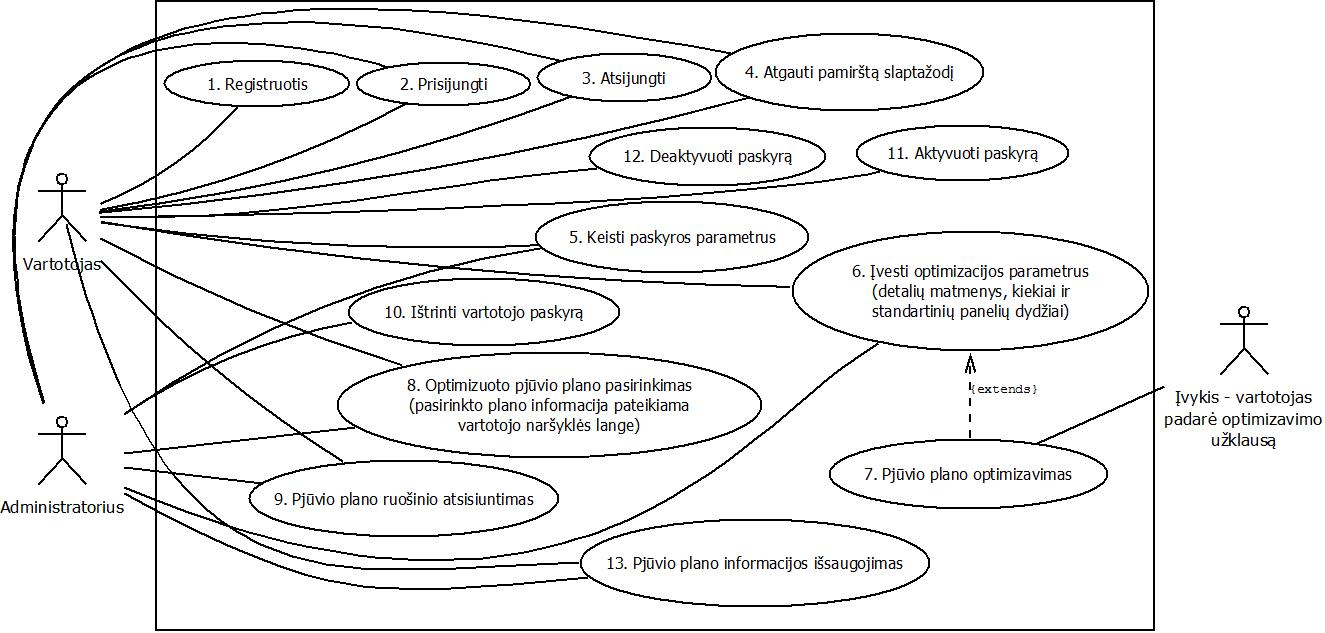
\includegraphics[width=180mm]{diagrama.jpeg}
\caption{A simple caption \label{overflow}}
\end{figure}

% <<<<<<<<<<<<<<<<<<<<<<<<<<<<ŠABLONO PABAIGA >>>>>>>>>>>>>>>>>>>>>>>>>>>>>>>>>>>>>>>>>>>>

\begin{frame}
\centering
\hspace{-1cm}
\label{my-label}
\begin{tabular}{|l|l|}
\hline
\textbf{Pavadinimas}  		& Registracija 							\\ \hline
\textbf{Dalyviai}  			& Vartotojas								\\ \hline
\textbf{Paskirtis}  			& Sukurti naujo vartotojo paskyrą		\\ \hline
\textbf{Kritiškumas}			& Būtinas 								\\ \hline
\textbf{Pradinės sąlygos}   	& Atidaryti tinklapy naršyklėje			\\ \hline
\textbf{Rezultatas}   		& Sistemos duomenų bazėje sukurtas 
							naujo vartotojo įrašą,vartotojas					\\ \hline
\textbf{
	\begin{tabular}[c]{@{}l@{}}
		Tipinė eiga ir kiti\\ 
		galimi variantai
	\end{tabular}
} &   
\begin{tabular}[c]{@{}l@{}}
	1. Vartotojas atidaręs P.O. tinklapy prieš naudojantis juo turi prisiregistruoti.\\
	Visų pirmą registravimosi formoje turi užpildyti	privalomus laukus: \\
		Unikalų vartotojo vardą ir unikalų, galiojantį el.paštą, slaptažodį.\\
	2. Suvedus duomenis paspausti mygtuką.\\
	3. Jeigu suvestas vartotojo vardas, bei paštas unikalus duomenų bazėje,\\
	tada sukuriamas vartotojo įrašas duomenų bazėje ir vartotojas\\
	nukreipiamas į jo naujos paskyros langą. \\
	Kitu atveju vartotojui pranešama, kad reikia įvesti iš naujo, \\
	nes suvestas paštas ir ar vardas pasikartojo.
\end{tabular} \\ \hline

\end{tabular}
\end{frame}

\vspace{2cm}

\begin{frame}
\centering
\hspace{-1cm}
\label{my-label}
\begin{tabular}{|l|l|}
\hline
\textbf{Pavadinimas}  		&	Prisijungimas 									\\ \hline
\textbf{Dalyviai}  			&	Vartotojas, administratorius					\\ \hline
\textbf{Paskirtis}  		&	Prieiga prie vartotojo paskyros, P.O. 			\\ \hline
\textbf{Kritiškumas} 		&	Būtinas											\\ \hline
\textbf{Pradinės sąlygos}	&	Naudotojo įrašas sistemos duomenų bazėje		\\ \hline
\textbf{Rezultatas}			&  	Prieiga prie savo paskyros bei P.O. atlikimas	\\ \hline
\textbf{
	\begin{tabular}[c]{@{}l@{}}
		Tipinė eiga ir kiti\\ galimi variantai
	\end{tabular}} 				&   
\begin{tabular}[c]{@{}l@{}}
1. Prisijungimo lange suvesti prisijungimo duomenis:\\ 
vartotojo vardą arba paštą ir slaptažodį.\\
2. Paspausti prisijungimo mygtuką.\\ 
3. Sistema patikrina ar prisijungimo duomenys atitinka naudotojo įrašo\\
duomenis(vardą ar paštą ir slaptažodį) duomenų bazėje.\\
Naudotojas nukreipiamas į savo paskyrą jei įvesti duomenys atitiko.\\
Kitu atveju pranešama, jog prisijungimo duomenys klaidingi,\\
lieka bandyti dar 2 kartus prisijungti iš naujo.
\end{tabular} \\ \hline

\end{tabular}
\end{frame}



\begin{frame}
\centering
\hspace{-1cm}
\label{my-label}
\begin{tabular}{|l|l|}
\hline
\textbf{Pavadinimas}		&	Atsijungimas nuo sistemos 						\\ \hline
\textbf{Dalyviai}			&   Vartotojas, administratorius    				\\ \hline
\textbf{Paskirtis}			&  	Nutraukti sistemos naudojimosi sesiją       	\\ \hline
\textbf{Kritiškumas}		&  	Mažas											\\ \hline
\textbf{Pradinės sąlygos}	& 	Sistemos naudotojas yra prisijungęs 
								prie sistemos   								\\ \hline
\textbf{Rezultatas}			&	Nutraukta sistemos naudotojo sesija      
\\ \hline
\textbf{
\begin{tabular}[c]{@{}l@{}}
	Tipinė eiga ir kiti\\ 
	galimi variantai
\end{tabular}} &
\begin{tabular}[c]{@{}l@{}}
	1. Sistemos naudotojas paspaudžia atsijungimo mygtuką, \\
	jo sesija sustabdoma.
\end{tabular} \\ \hline
\end{tabular}
\end{frame}

\vspace{1cm}

\begin{frame}
\centering
\hspace{-1cm}
\label{my-label}
\begin{tabular}{|l|l|}
\hline
\textbf{Pavadinimas}		&  	Slaptažodžio atgavimas					\\ \hline
\textbf{Dalyviai}			&	Vartotojas, administratorius			\\ \hline
\textbf{Paskirtis}			&   Sužinoti pamirštą slaptažodį.			\\ \hline
\textbf{Kritiškumas}		&	Būtinas 								\\ \hline
\textbf{Pradinės sąlygos}	&  								 			\\ \hline
\textbf{Rezultatas}			&	\begin{tabular}[c]{@{}l@{}}
								Naudotojas į el. paštą gauna savo \\
								slaptažodžio priminimą
								\end{tabular}   						\\ \hline
\textbf{
	\begin{tabular}[c]{@{}l@{}}
		Tipinė eiga ir kiti\\ 
		galimi variantai
	\end{tabular}
} &   
\begin{tabular}[c]{@{}l@{}}

	1. Paspaudžiamas pamiršto slaptažodžio atgavimo mygtukas.\\
	2. Atsidariusioje formoje nurodomas el. paštas\\ 
	ar vardas, kurie yra užregistruoti sistemoje.\\ 
	3. Paspaudžiamas mygtukas ir vykdoma forma. \\
	4. Jei el. paštas ar vardas egzistuoja sistemos duomenų bazėje, tada bus\\ 
	nusiunčiamas laiškas su slaptažodžiu į naudotojo įraše esantį paštą . \\

	Jei nei vardo, nei el. pašto atitikmens nerandama \\
	duomenų bazėje, perspėjama, kad įvesti duomenys klaidingi \\
	ir pasiūloma prisiregistruoti.
\end{tabular} \\ \hline

\end{tabular}
\end{frame}

\begin{frame}
\centering
\hspace{-1cm}
\label{my-label}
\begin{tabular}{|l|l|}
\hline
\textbf{Pavadinimas}		&  	Įvedami pjovimo detalių ir panelių optimizacijos parametrai.		\\ \hline
\textbf{Dalyviai}			&  	Vartotojas, administratorius  					\\ \hline
\textbf{Paskirtis}			&  	\begin{tabular}[c]{@{}l@{}}
									Parametrų perdavimas, pagal kuriuos algoritmas optimizuos detales \\
									ant standartinių  panelių
								\end{tabular}									\\ \hline
\textbf{Kritiškumas}		& 	Būtinas											\\ \hline
\textbf{Pradinės sąlygos}	& 	Naudotojas yra prisijungęs ir atsidaręs pjovimo optimizavimui skirtą formą \\ \hline
\textbf{Rezultatas}			& 	\begin{tabular}[c]{@{}l@{}}
									Įvesti reikalingus parametrus optimizacijos vykdymui. \\
								\end{tabular} \\ \hline
\textbf{
	\begin{tabular}[c]{@{}l@{}}
		Tipinė eiga ir kiti\\ galimi variantai
	\end{tabular}
} &   
\begin{tabular}[c]{@{}l@{}} 
	1. Optimizacijos formoje suteikiami pasirenkami standartiniai panelių \\
	dydžiai(1200x2500, 1200x3050), prie jų galima įvesti norimų standartinių \\
	panelių	matmenis. Optimizacija galės vykti tik tada kai bus nurodyta ar įvesta \\
	bent viena panelė.\\
	
	2. Taip pat vartotojas nurodomi reikalingų detalių ilgiai (mm),\\ 
	aukščiai (mm) ir kiekiai. Taip pat galima įkelti xlsx formato failą, \\
	kuriame yra du stulpeliai ilgis ir plotis, o po jais N detalių matmenų, \\
	kurioms bus atliekama optimizacija. Detalių duomenys nurodomi sveikaisiais \\
	skaičiais ir jų ilgiai aukščiai atitinkamai mažesni arba lygūs nurodytom \\
	standartinėm panelėm. Optimizacija vyks tik tada, jei viskas įvesta teisingai.\\
	
\end{tabular} \\ \hline

\end{tabular}
\end{frame}

\vspace{1cm}

\begin{frame}
\centering
\hspace{-1cm}
\label{my-label}
\begin{tabular}{|l|l|}
\hline
\textbf{Pavadinimas}			&  	Įvesti papildomus standartinių panelių dydžius		\\ \hline
\textbf{Dalyviai}			&  	Vartotojas, administratorius  						\\ \hline
\textbf{Paskirtis}			&  	Nurodyti papildomą standartinės panelės dydį.				\\ \hline
\textbf{Kritiškumas}			& 	Būtinas												\\ \hline
\textbf{Pradinės sąlygos}	& 	\begin{tabular}[c]{@{}l@{}}
									Naudotojas yra prisijungęs ir atsidaręs pjovimo optimizavimui skirtą langą.\\ 
									bei prie pasirenkamų standartinių panelių dydžių paspausti mygtuką "Naujas". \\
								\end{tabular}  \\ \hline
\textbf{Rezultatas}			&  	\begin{tabular}[c]{@{}l@{}}
									Naudotojas turi galimybę nurodyti panelių, iš kurių nori pjauti detales,\\ dydį\end{tabular} \\ \hline
\textbf{\begin{tabular}[c]{@{}l@{}}Tipinė eiga ir kiti\\ galimi variantai\end{tabular}} &   \begin{tabular}[c]{@{}l@{}} 1. Vartotojas peržiuri siūlomų panelių dydžių sąrašą. Optimizacijai \\gali pasirinkti vieną iš šių siūlomų variantų arba nurodyti kitokius \\matmenis. Antruoju atveju būtų taikomi įvedamų matmenų apribojimai,\\pavyzdžiui, matmuo negali būti didesnis negu 5000mm ar mažesnis\\ negu 2000mm. \end{tabular} \\ \hline
\end{tabular}
\end{frame}

\begin{frame}
\centering
\hspace{-1cm}
\label{my-label}
\begin{tabular}{|l|l|}
\hline
\textbf{Pavadinimas}                                                                    &  Optimizuoto pjūvio plano pasirinkimas\\ \hline
\textbf{Dalyviai}                                                                       &   Vartotojas    \\ \hline
\textbf{Paskirtis}                                                                      &  
\begin{tabular}[c]{@{}l@{}}
Leisti vartotojui pasirinkti, kuris pjūvio optimizacijos planas \\ jam labiau priimtinas 
\end{tabular}  \\ \hline
\textbf{Kritiškumas}                                                                    & Būtinas\\ \hline
\textbf{Pradinės sąlygos}                                                               & 
\begin{tabular}[c]{@{}l@{}}
Vartotojas yra prisijungęs. Sistema baigusi optimizuoti pjūvio \\planus/planą pagal vartotojo nurodytus optimizacijos parametrus \\optimizacijos lange. Priklausomai nuo optimizacijos parametrų \\vartotojas gauna nuo vieno iki triejų skirtingų pjovimo\\ optmizacijos planų
\end{tabular} \\ \hline
\textbf{Rezultatas}                                                                     &   \begin{tabular}[c]{@{}l@{}} Vartotojas savo naršyklės lange mato vieną, detalų pjovimo\\optimizacijos planą ir turi galimybę jį atsispausdinti\end{tabular}     \\ \hline
\textbf{\begin{tabular}[c]{@{}l@{}}Tipinė eiga ir kiti\\ galimi variantai\end{tabular}} &   \begin{tabular}[c]{@{}l@{}} 1. Vartotojas pasirenka vieną iš jam pateiktų pjovimo planų\\ ir patvirtina, jog nori matyti konkretų planą.\\2. Vartotojo naršyklės lange atsiranda detalus, pasirinktasis\\ pjovimo planas ir mygtukas, leidžiantis vartotojui parsisiųsti,\\ spausdinimui skirtą plano kopiją. Pastarasis planas \\ bus saugomas sistemos duomenų bazėje visam laikui, kai, tuo \\tarpu, nepasirinktieji optimizuoti pjovimo planai yra saugomi\\ sistemos duomenų bazėje iki vartotojo sesijos pabaigos.\end{tabular} \\ \hline
\end{tabular}
\end{frame}

\begin{frame}
\centering
\hspace{-1cm}
\label{my-label}
\begin{tabular}{|l|l|}
\hline
\textbf{Pavadinimas}                                                                    &  Pasirinkto pjūvio plano ruošinio gavimas\\ \hline
\textbf{Dalyviai}                                                                       &   Vartotojas    \\ \hline
\textbf{Paskirtis}                                                                      &  
\begin{tabular}[c]{@{}l@{}}
Leisti vartotojui gauti spausdinimui skirtą pjūvio plano kopiją
\end{tabular}  \\ \hline
\textbf{Kritiškumas}                                                                    & Būtinas\\ \hline
\textbf{Pradinės sąlygos}                                                               & 
\begin{tabular}[c]{@{}l@{}}
Vartotojas yra prisijungęs. Sistema baigusi optimizuoti pjūvio \\planus/planą pagal vartotojo nurodytus optimizacijos parametrus \\optimizacijos lange. Vartotojas yra pasirinkęs pjūvio optimizavimo\\ planą, kurį nori atsispausdinti
\end{tabular} \\ \hline
\textbf{Rezultatas}                                                                     &   \begin{tabular}[c]{@{}l@{}} Vartotojas savo prietaise turės spausdinimui paruoštą\\ pjūvio planą\end{tabular}     \\ \hline
\textbf{\begin{tabular}[c]{@{}l@{}}Tipinė eiga ir kiti\\ galimi variantai\end{tabular}} &   \begin{tabular}[c]{@{}l@{}} 1. Vartotojas paspaudžia mygtuką, skirtą gauti spausdinimui \\paruoštą planą.\\2. Į vartotojo prietaisą atsiunčiamas pjuvio planas.\end{tabular} \\ \hline
\end{tabular}
\end{frame}

\begin{frame}
\centering
\hspace{-1cm}
\label{my-label}
\begin{tabular}{|l|l|}
\hline
\textbf{Pavadinimas}			&  	Keisti paskyros parametrus						\\ \hline
\textbf{Dalyviai}			&	Vartotojas, administratorius					\\ \hline
\textbf{Paskirtis}			&	Leisti vartotojui keisti savo paskyruos duomenis	\\ \hline
\textbf{Kritiškumas}			& 	Vidutinis\\ \hline
\textbf{Pradinės sąlygos}	&  	Vartotojas ar administratorius 
								turi būti prisijungęs							\\ \hline
\textbf{Rezultatas}			&   Pasikeitę vartotojo paskyros parametrai        	\\ \hline
\textbf{
\begin{tabular}[c]{@{}l@{}}
	Tipinė eiga ir kiti\\ galimi variantai
\end{tabular}
} &   
\begin{tabular}[c]{@{}l@{}} 
	1. Vartotojas spaudžia paskyros redagavimo mygtuką.\\ 
	2. Vartotojas pakeičia norimus paskyros duomenis.\\ 
	3. Vartotojas spaudžia pakeitimų išsaugojimo mygtuką.\\
	4. Jei pakeitimai buvo leistini, pavyzdžiui, vartotojo\\ 
	vardas nebuvo pakeistas į tuščią reikšmę ir pan., tada \\
	pakeitimai išsaugomi. Kitu atveju pažymimi\\ 
	neleistinas reikšmes įgiję laukai. Vartotojas jas turi \\
	pakeisti, kad galėtų išsaugoti pakitimus.
\end{tabular}																	 \\ \hline

\end{tabular}
\end{frame}

\vspace{1cm}

\begin{frame}
\centering
\hspace{-1cm}
\label{my-label}
\begin{tabular}{|l|l|}
\hline
\textbf{Pavadinimas}		&  	Išrinti vartotojo paskyrą 									\\ \hline
\textbf{Dalyviai}			&	Vartotojas						\\ \hline
\textbf{Paskirtis}			&	Ištrinti nenaudojamas ar kenkėjiškas paskyras	\\ \hline
\textbf{Kritiškumas}		& 	Būtinas											\\ \hline
\textbf{Pradinės sąlygos}	& 	Vartotojas 
								turi būti prisijungęs							\\ \hline
\textbf{Rezultatas}			&   Ištrintas tam tikras vartotojo įrašas        	\\ \hline
\textbf{
\begin{tabular}[c]{@{}l@{}}
	Tipinė eiga ir kiti\\ galimi variantai
\end{tabular}} &   
\begin{tabular}[c]{@{}l@{}} 
	1. Vartotojas spaudžia paskyros redagavimo mygtuką.\\ 
	2. Vartotojas pakeičia norimus paskyros duomenis.\\ 
	3. Vartotojas spaudžia pakeitimų išsaugojimo mygtuką.\\
	4. Jei pakeitimai buvo leistini, pavyzdžiui, vartotojo\\ 
	vardas nebuvo pakeistas į tuščią reikšmę ir pan., tada \\
	pakeitimai išsaugomi. Kitu atveju pažymimi\\ 
	neleistinas reikšmes įgiję laukai. Vartotojas jas turi \\
	pakeisti, kad galėtų išsaugoti pakitimus.
\end{tabular}																	 \\ \hline

\end{tabular}
\end{frame}

\section{Sistemos elgsenos aprašymas}



\end{document}
>>>>>>> 47578c9659969186db316aec067e431147956cc0
